\section{Background}
\label{sec:background}

% MDPs
In reinforcement learning, the standard representation of an environment
and task instance is a Markov decision process (MDP). An MDP can be
represented as the tuple, $\tuple{ \states, \actions, \transitions,
\rewards, \gamma }$, where $\states$ and $\actions$ are finite sets of
states and actions, $\transitions: \states \times \actions \times
\states \to [0,1]$ describes the dynamics of the world through
state-action transition probabilites, $\rewards: \states \times \actions
\to \Re$ describes the task at hand by ascribing rewards for state
transitions, and $\gamma \in [0,1]$ is a discount factor that weighs the
value of future rewards.

In this setting, an agent in a state $s \in \states$ chooses an action
$a \in \actions$, and moves to a state $s'$ with probability
$\transitions(s,a,s')$, receiving a reward $\rewards(s,s')$. The
objective of the agent is to find a policy $\pi: \states \times \actions
\to [0,1]$, i.e. a decision procedure for selecting actions, that
maximises the reward it accumulates in the long run, $R = \sum_{i}
\gamma^i r_i$. $R$ is also called the return.

We define the value function $Q: \states \times \actions \to \Re$ to be
the expected return after taking the action $a$ from $s$. The optimal
value function must satisify the Bellman equation, 
\begin{eqnarray*}
  Q(s,a) &=& \rewards(s,a) + \gamma \sum_{s' \in \states} \transitions(s,a,s') \max_{a'} Q(s',a').
\end{eqnarray*}

Given an optimal $Q$, an agent can construct an optimal policy,
$\pi(s,a^*) = 1$ when $a^* = \argmax_{a} Q(s,a)$, and $0$ otherwise. In
principle, if the agent knew the MDP, it could construct the optimal
value function, and from it an optimal policy.  However, in the usual
setting, the agent is only aware of the state-action space, $\states$
and $\actions$, and must learn $Q$ through exploration. The Q-learning
algorithm learns $Q$ with a simple update for every step the agent
takes, 
\begin{eqnarray*}
    Q(s,a) &=& Q(s,a) + \alpha [ r + \gamma \max_{a'} Q(s',a') - Q(s,a) ],
\end{eqnarray*}
\noindent
where $\alpha \in [0,1]$ is a parameter that controls the learning rate.
It has been shown that the Q-learning algorithm converges to the optimal
value function in the limit with fairly permissive assumptions.

% Options
The options framework provide a temporal abstraction for subtasks. An
option $\option$ is described by an initiation set $\initset \subset
\states$, a policy $\pi$, and a terminating condition $\beta$.  An agent
can exercise an option in any state $s \in \initset$, following which,
it will follow the policy $\pi$ described by the option, until the
terminating condition $\beta(s)$ is satisfied. The terminating condition
$\beta$ can be stochastic.

Several learning algorithms have been proposed for agents using options
\cite{SuttonPrecupSingh1999,BartoMahadevan2003}. One simple such method that
we will use is MacroQ, a generalisation of the Q-learning algorithm
described above. The MacroQ algorithm updates the value function only
after completion of the option. If the option $o$ was initiated in the
state $s$, and continues for $k$ steps before terminating in $s'$, the
corresponding $Q$ function update will be,
\begin{eqnarray*}
    Q(s,o) &=& Q(s,o) + \alpha [ r + \gamma^{k} \max_{o' \in \actions \cup \options} Q(s',o') - Q(s,o) ].
\end{eqnarray*}

Different tasks in the same domain can be described by different
$\rewards$. Let $\rewards$ be sampled from the family $\Rewards$. Our
objective then is to find a set of options $O$ that reduces the expected
learning time over $\Rewards$.

\begin{figure*}[th]
    \center
    \subfigure{
      \documentclass{article}
\usepackage{tikz}
\usetikzlibrary{external}
\usetikzlibrary{arrows}
%\tikzexternalize % activate!

\begin{document}
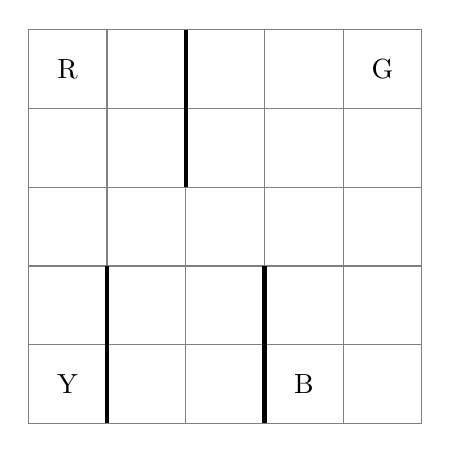
\begin{tikzpicture}
    % Grid
    \draw[step=1,color=gray] (0,0) grid (5,5);
    
    % Walls
    \draw[line width=1.5pt] (2,5) -- (2,3);
    \draw[line width=1.5pt] (1,0) -- (1,2);
    \draw[line width=1.5pt] (3,0) -- (3,2);

    % Pads
    \draw (0.5,4.5) node {R};
    \draw (0.5,0.5) node {Y};
    \draw (3.5,0.5) node {B};
    \draw (4.5,4.5) node {G};
\end{tikzpicture}
\end{document}

      \label{fig:taxi-domain}
    }
    \subfigure{
      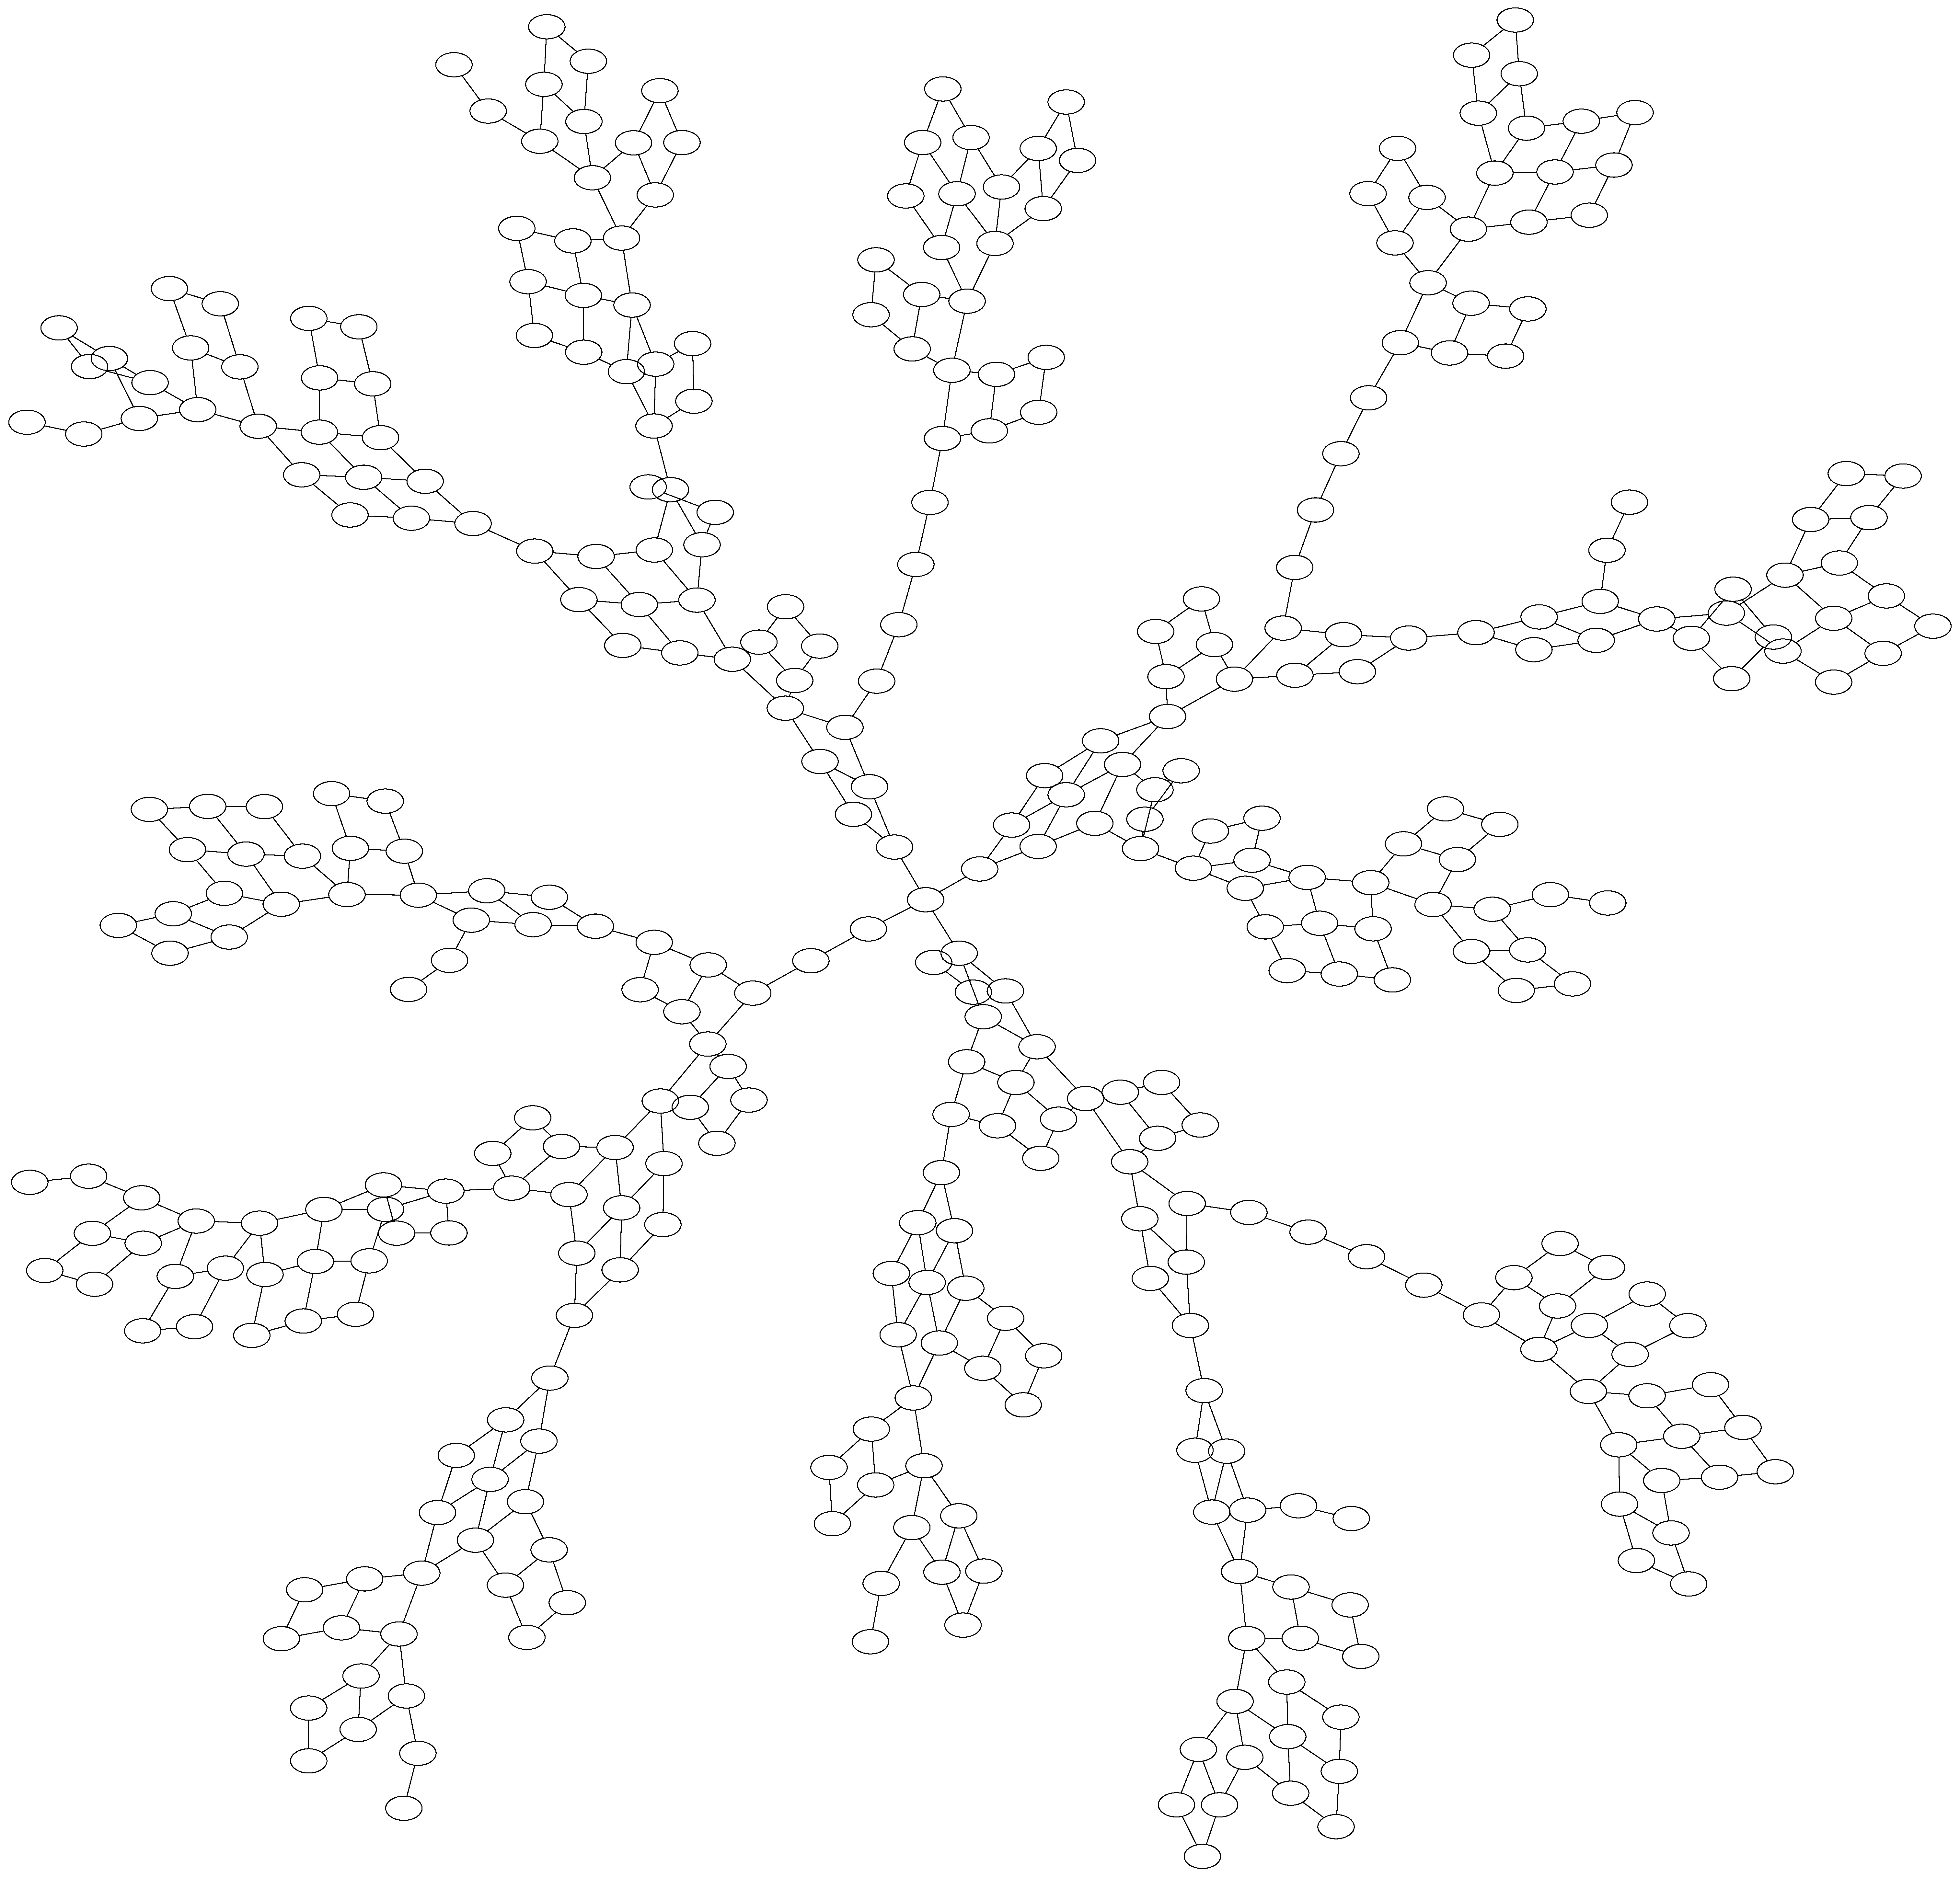
\includegraphics[height=2in]{figures/taxi1}
      \label{fig:taxi-graph}
    }
    \caption{The Taxi Domain, and its State Space Graph}
\end{figure*}

\begin{example}
  \label{example:taxi}
To make the discussion more tangible, let us look at an example, the
Taxi domain, shown in \figref{fig:taxi-domain}. The agent is a taxi
navigating in this road-map. It must pick up a passenger at one of the
4 pads, A, B, C or D.  Subsequently, it must carry the passenger to a
destination, which is also one of the above four pads. The states of
the taxi would then be a tuple containing the location of the
passenger (in one of the four pads, or within the taxi), the
destination of the passenger, and location of the taxi in the map.
The actions the taxi can perform are moving up, down, left or right in
the map, as well as pick up or drop a passenger at a pad. 
Typical options for such a domain would be an option that can be
started anywhere, and has a policy that takes the taxi to the one of
the pads in the shortest possible manner. Such an option is generic,
and does not depend on where the passenger or destination are. The RL
agent must then learn to choose the right option when picking up the
passenger.
\end{example}

